%%%%%%%%%%%%%%%%%%%%%%%%%%%%%%%%%%%%%%%%%%%%%%%%%%%%%%%%%%%%%%%%%%%%%%%%%%%%%
%%%                                Table                                  %%%
%%%%%%%%%%%%%%%%%%%%%%%%%%%%%%%%%%%%%%%%%%%%%%%%%%%%%%%%%%%%%%%%%%%%%%%%%%%%%
\subsubsection{Table}
The user interface element \TABLE{}
is a multi-purpose widget for displaying and editing matrices and lists.

\label{sec:uitable}
\input{diagrams/ui_table_list}
\index{TABLE@\TABLE!ui\_manager table declaration}

The table options define the behaviour and appearance
of the table.

\input{diagrams/ui_tbl_option}
\index{justify!ui\_manager table option}
\index{JUSTLEFT@\JUSTLEFT!ui\_manager table option}
\index{JUSTRIGHT@\JUSTRIGHT!ui\_manager table option}
\index{CENTER@\CENTER!ui\_manager table option}
\index{ORIENTATION@\ORIENTATION!ui\_manager table option}
\index{NAVIGATION@\NAVIGATION!ui\_manager table option}
\index{HORIZONTAL@\HORIZONTAL!ui\_manager table option}
\index{VERTICAL@\VERTICAL!ui\_manager table option}
\index{MENU@\MENU!UI\_MANAGER!TABLE MENU=HIDDEN}
\index{HIDDEN@\HIDDEN!table option \MENU=\HIDDEN}
\index{FUNC@\FUNC!ui\_manager table option}
\index{AUTOWIDTH@\AUTOWIDTH!ui\_manager table option}

\begin{tabularx}{\textwidth}{l|X}
option              & description \\
\hline
{\verb+string+}     & The title of the table\\
\JUSTLEFT           & TODO\\
\JUSTRIGHT          & TODO\\
\CENTER             & Without one of these options, \INTENS{} places the table fields left
                      justified within each column. \\
\ORIENTATION        & The tables default orientation is horizontal. \\
\NAVIGATION         & determines the direction in which the tables
                      text fields are to be traversed during keyboard navigation.
                      \HORIZONTAL{} is the default value.\\
\HORIZONTAL         & horizontal size and range \\
\VERTICAL           & vertical size and range \\
\MENU{} = \HIDDEN   & Do not display table row/column menu, when right mouse button is pressed at row/column header.
                      (See section \nameref{par:uitablemenurowcolumn} on page \pageref{par:uitablemenurowcolumn}.) \\
\FUNC               & function to call by mouse click or enter key \newline
                      The function can use a \nameref{fuexpressionsreason} (see page \pageref{fuexpressionsreason})
                      to distinguish select, unselect, ... \\
\AUTOWIDTH          & tell webtens to determine the column widths automatically,
                      based on the content \\
\end{tabularx}


\input{diagrams/ui_tbl_size_options}
\index{TABLESIZE@\TABLESIZE!table direction option}
\index{RANGE@\RANGE!table direction option}
\index{HIDDEN@\HIDDEN!table direction option}
\index{SCROLLBARS@\SCROLLBARS!use \RANGE{} to hide \SCROLLBAR{} in \TABLE}

\begin{tabularx}{\textwidth}{l|X}
size options        & description \\
\hline
\TABLESIZE          & defines the minimal number of rows (\VERTICAL) or columns (\HORIZONTAL)
                      shown in the \TABLE{} part. \newline
                      \TOP{} and \BOTTOM{} rows are shown in addition. \newline
                      \LEFT{} and \RIGHT{} columns are shown in addition. \\
\RANGE              & determines the index range that can be used for the associated
                      data items. The default starting index is 0. \newline
                      The first number defines the number shown for index 0.
                      It is the offset of the number shown on the gui. \newline
                      The optional second index is the maximal number shown. \newline
                      The second index also defines the maximal number of data items shown.
                      When that number is less than or equal \TABLESIZE, the \SCROLLBAR{} is not shown. \\
\HIDDEN             & \HORIZONTAL{} or \VERTICAL{} headers are not shown  \\
\end{tabularx}

\newpage
\input{diagrams/ui_tbl_part}
\index{TABLE@\TABLE!ui\_manager table entries}
\index{TOP@\TOP!ui\_manager table}
\index{BOTTOM@\BOTTOM!ui\_manager table}
\index{LEFT@\LEFT!ui\_manager table}
\index{RIGHT@\RIGHT!ui\_manager table}

\begin{tabularx}{\textwidth}{l|X}
option                  & description \\
\hline
\TOP                    & positions following lines at the top of the table. \\
\BOTTOM                 & positions following lines at the bottom of the table. \\
\LEFT                   & positions following lines to the left of the table. \\
\RIGHT                  & positions following lines to the right of the table. \\
\TABLE                  & specifies the table entries (data displayed in the table) \\
{\verb+title string+}   & The title of the specified side of the table \\
\end{tabularx}


\newpage
\input{diagrams/ui_tbl_table_line_list}
\input{diagrams/ui_tbl_horizontal_line_list}
\input{diagrams/ui_tbl_line_item}
\input{diagrams/ui_tbl_table_matrix}
\index{alignment!ui\_manager table}
\index{MATRIX@\MATRIX}
\index{VOID@\VOID!ui\_manager table}
\index{TOOLTIP@\TOOLTIP!ui\_manager table}
\index{COLOR@\COLOR!ui\_manager table}

\begin{tabularx}{\textwidth}{l|X}
  table items               & description \\
\hline
\VOID                     & creates an empty space. \\
\TOOLTIP                  & The values of this row/column are not shown but used as the tooltips. \\
\COLOR                    & The values of this row/column are not shown.
                            The colors corresponding to their values
                            (see section \nameref{sec:dpcolorset} on page \pageref{sec:dpcolorset})
                            are used for the column/row. \\
{\verb+string+}           & A label string. Defines the colum/row header. \\
{\verb+alignment+}        & (see section \nameref{dia:uifieldalignment} on page \pageref{dia:uifieldalignment}) \\
{\verb+data reference+}   & (see section \nameref{dia:uifielddatareference} on page \pageref{dia:uifielddatareference}) \\
{\verb+field attributes+} & (see section \nameref{dia:uifieldattributes} on page \pageref{dia:uifieldattributes}) \newline
                              To hide a column, provide a width of 0 \newline
                              Hiding a column is useful when table row/column menu (right mouse button)
                              are used. The menu functions delete, insert, clear etc. all fields in the table.
                              This includes hidden columns. \\
\end{tabularx}

\newpage
The following example shows the configuration of two tables
and how they will be displayed by \INTENS{} (see page \pageref{fig:tables})

\begin{boxedminipage}[ht]{\linewidth}
\begin{alltt}
  \TABLE
    Table1 \{ "Table 1"
           , \HORIZONTAL ( \TABLESIZE = 5  )
           , \VERTICAL   ( \TABLESIZE = 23 )
           \}
    ( \TOP   ( "Length"  length[0:*,0]:10
             , "Weight"  weight[0:*,1]:10
             );
      \LEFT  ( "Speed"   speed[0:*]:10     );
      \TABLE ( rslt[*,*]:10 );
    )
  , Table2 \{ "Table 2"
           , \HORIZONTAL ( \TABLESIZE = 3 )
           , \ORIENTATION = \HORIZONTAL
           , \NAVIGATION  = \HORIZONTAL
           \}
    ( \TOP ( "Color"   color[0,*]:-20     );
      \TABLE ( "first"   first [0,*]:-10
             , "second"  second[1,*]:10
             , "third"   third [2,*]:10   );
    )
  ;
\end{alltt}
\end{boxedminipage}

\vspace{1cm}

\begin{figure}[H]\label{fig:tables}
  \begin{center}
    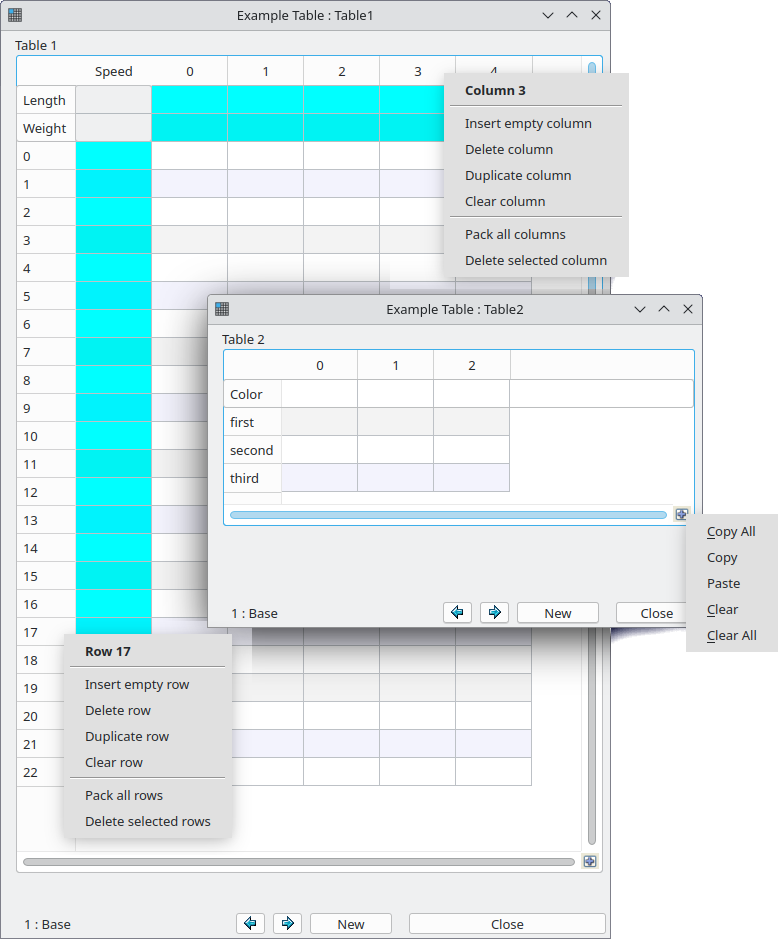
\includegraphics[width=300px]{grab_table}
  \end{center}
\caption{example of \TABLE}
\end{figure}

\paragraph{\TABLE{} menus}
\label{par:uitablemenu}

\INTENS{} \TABLE{}s have two kind of right click menus:

\subparagraph{row/column menu}
\label{par:uitablemenurowcolumn}

These menus are shown when the right mouse button is pressed on a row or column header.
The menu header shows the type of menu (Row or Column) and number of the row/column the menu was opened for.
The first four entries depend on that row/column number.

\begin{tabularx}{\textwidth}{l|X}
  row menu entries        & description \\
\hline
Insert empty row          & An empty row is inserted.
                            This shifts down the values of this and all following rows. \\
Delete row                & The row is deleted.
                            This shifts up the values of all following rows. \\
Duplicate row             & A new row with the values of this row is inserted.
                            This shifts down the values of this and all following rows. \\
Clear row                 & The values of this row are deleted, but the row is kept. \\
\hline
Pack rows                 & Values are shifted up to fill empty cells. \\
Delete selected rows      & This is independent of the row the menu is shown for.
                            It deletes the rows of all selected table cells.
                            Following rows are shifted up. \\
\end{tabularx}

\begin{tabularx}{\textwidth}{l|X}
  column menu entries     & description \\
\hline
Insert empty column       & An empty column is inserted.
                            This shifts right the values of this and all following columns. \\
Delete column             & The column is deleted.
                            This shifts left the values of all following columns. \\
Duplicate column          & A new column with the values of this column is inserted.
                            This shifts right the values of this and all following columns. \\
Clear column              & The values of this column are deleted, but the column is kept. \\
\hline
Pack columns              & Values are shifted left to fill empty cells. \\
Delete selected columns   & This is independent of the column the menu is shown for.
                            It deletes the columns of all selected table cells.
                            Following columns are shifted left. \\
\end{tabularx}

\subparagraph{bottom right menu}
\label{par:uitablemenubottomright}

This menu is shown when the right mouse button is pressed on the cross at bottom right corner of the table.

\begin{tabularx}{\textwidth}{l|X}
  corner menu entries     & description \\
\hline
Copy All                  & All values are copied to the clipboard,
                            i.E. to be pasted into a spreadsheet or another \INTENS \TABLE. \\
Copy                      & The selected values are copied,
                            i.E. to be pasted into a spreadsheet or another \INTENS \TABLE. \\
Paste                     & Previously copied values are pasted to the table, starting at the selected cell. \\
Clear                     & The selected values are deleted. \\
Clear All                 & All values are deleted. \\
\end{tabularx}

Paste and Clear operations are done cell by cell, as if the user would change the values.
Therefore, the variables functions (if any) is called with \REASONINPUT, \INPUT, \OLDVALUE, \INDEX, \NODE, \THIS, etc.
available inside the functions.
